\chapter{Recent trends and natural variability}
\label{cha:SHcirc}

\begin{quotation}
  The work contained in this chapter is based upon \citet{Thomas2015},
  published in \emph{Geophysical Research Letters}.
\end{quotation}

\section{Overview and aims}

The Southern Ocean plays a critical role in the ocean overturning circulation
and moderating global climate through carbon and heat uptake
\citep{Khatiwala2009,Gnanadesikan1999}, with approximately 40$\%$ of
anthropogenic carbon and 75$\%$ of heat entering the ocean south of 30$^\circ$S
\citep{Frolicher2015,Sabine2004}. The leading mode of Southern Hemisphere
(SH) extratropical variability, the Southern Annular Mode (SAM), has been shown
to directly affect this overturning circulation and the distribution of
anthropogenic carbon uptake by altering the magnitude and location of the
westerly jet \citep{Hall2002b,Mignone2006b,SenGupta2006e}.  It is
therefore important to understand the variability in the SH extratropical
circulation.

Observations and reanalyses have shown a positive trend in SAM and jet magnitude
over the last couple decades along with a poleward shift in the jet location
\citep{Thompson2000b,Thompson2002e} in addition to trends in subtropical sea
surface temperature, Antarctic sea ice extent, ocean ventilation and gyre
circulation \citep{Parkinson2012c,Swart2012a,Waugh2013b,Roemmich2007b}.
Additionally, studies have detected anthropogenic influences in surface pressure
and the westerly jet \citep{Gillett2003,Gillett2005}. These trends in the
SAM and consequently the jet have been largely attributed to ozone depletion in
the SH stratosphere during austral summer \citep{Previdi2014f,Gillett2013,
Gillett2003a}. However, there is also evidence that this positive phase trend
in the SAM is due in part to greenhouse gas warming \citep{Arblaster2006,
Lee2013f,Gillett2013}.

While there is evidence of anthropogenic forcing, understanding the forcing in
the context of natural variability is difficult given the lack of in-situ
observations and satellite information prior to 1979. Previous studies have
tried to quantify the natural variability in the SH using proxy records
\citep{MARSHALL2003,Visbeck2009} and climate models \citep{Latif2013}.
Understanding the relative contribution of natural variability and anthropogenic
forcing to recent trends is critical to understanding how global climate will be
influenced in the future.

In this study, we aim to further estimate the natural variability of the SH
extratropical circulation by using the Coupled Model Intercomparison Project
Phase 5 (CMIP5) pre-industrial control model runs. We examine five metrics of
the SH extratropical circulation: the SAM, the jet location defined using the
850mb winds ($U_{lat}$) and the surface wind-stress ($\tau_{lat}$), the jet
magnitude defined by the 850mb winds ($U_{max}$) and the surface wind-stress
($\tau_{max}$). We turn to CMIP5 pre-industrial model runs to quantify the
natural variability of these five metrics to address the following questions:
Can recently observed trends in SH circulation occur in CMIP5 piControl model
runs due to natural variability alone, do the CMIP5 models historical
(1980-2004) runs show significant trends in the circulation metrics, and do
these simulated historical trends capture the characteristics of the observed
trends?

\section{Methods}


In order to examine the natural multi-decadal-scale variability in the SH
circulation we use a combination of pre-industrial control (``piControl'') and
historical (1980 to 2004) runs from models. Table 1 lists the models used in
this study, the length of their piControl run and the number of historical runs.
The models were chosen based on the availability of monthly-mean fields of sea
level pressure, 850mb zonal winds and zonal wind-stress for both piControl and
historical runs.  We focused on the austral summer (averaged over December,
January and February) because this is the season where the largest trends are
observed \citep{Thompson2002e,Thompson2011}.

From the monthly sea-level pressure, we calculated the SAM as the zonal sea
level pressure difference between $65^{\rm o}$ and $40^{\rm o}$ degrees South.
For the sake of comparisons across different models, we chose to leave the SAM
as a surface pressure difference as opposed to normalizing by the standard
deviation as done in \citet{Gong1999} to avoid normalizing by different
standard deviations across models. Additionally, we examine the SH  westerly
jet magnitude and location calculated using both zonal surface wind-stress
($\tau_{max}$ and $\tau_{lat}$) and 850mb zonal winds ($U_{max}$ and $U_{lat}$).
To find the jet maximum and location, the maximum zonal-mean wind-stress/850mb
winds and the surrounding 4 grid-points were isolated and interpolated to a
0.1-degree meridional grid. A quadratic polynomial was then fit to the
interpolated data and the maximum magnitude and location was found.

%%% Table
{\small
\begin{table}[t]
\caption{CMIP 5 models used in this study.}
\centering
\begin{tabular}{ l p{5cm} p{5cm} }
\hline
 Model & piControl model run length (years) & Historical model ensemble  runs \\
\hline
 CanESM2 & 996 & 1\\
 %\hline
 CNRM CM5 & 850 & 10\\
 %\hline
 GFDL ESM2M & 500 & 1\\
 %\hline
 IPSL CM5a LR & 1000 & 6\\
 %\hline
 IPSL CM5a MR & 300 & 3\\
 %\hline
 IPSL CM5b LR & 300 & 1\\
 %\hline
 MIROC ESM & 531 & 3\\
 %\hline
 MIROC ESM CHEM & 255 & 1\\
 %\hline
 MIROC5 & 200 & 5\\
 %\hline
 MPI ESM LR & 1000 & 3\\
 %\hline
 MPI ESM MR & 1000 & 3\\
 %\hline
 MRI CGCM3 & 500 & 3\\
 %\hline
 NOR ESM1m M & 501 & 1\\
 %\hline
 NOR ESM1m ME & 252 & 1\\
\hline
\end{tabular}
\end{table}
}
%%% End Table

While there are no trends (i.e., drift) in these metrics over the length of the
piControl time-series (order 250-1000 years), strong multi-decadal trends are
found. Time-series in SAM from a high-varying model (MPI ESM MR) and a
low-varying model (MIROC5) are shown in Figure~\ref{fig:ch2_fig1}a and c
respectively. As highlighted in red, there are multiple 25-year periods that
have strong trends even though there is no trend over the entire time-series.
In order to quantify the variability of these multi-decadal-scale trends, we
calculate the linear trend of each metric (SAM, $\tau_{max}$, $\tau_{lat}$,
$U_{max}$, and $U_{lat}$) for consecutive and overlapping 25-yr trends for each
model's piControl run (\citet{Polvani2013e} performed a similar analysis for
sea ice extent in piControl runs).

\begin{figure}[t]
\noindent
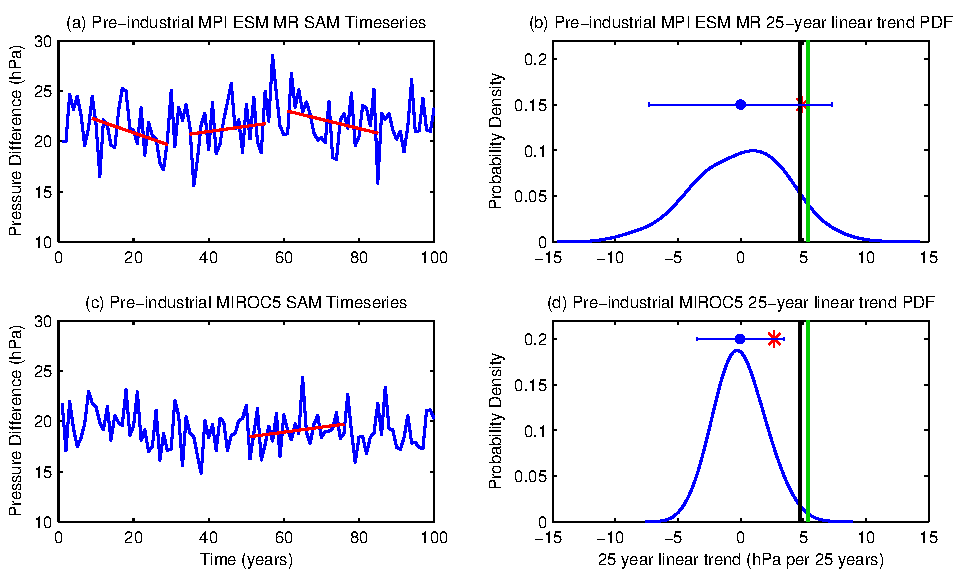
\includegraphics[width=\linewidth]{figures/chapter-SHcirc/2014jgrl-p01.pdf}
\caption{SAM time-series for (a) MPI ESM MR and (c) MIROC5 piControl runs over
the first 100 years. The red lines indicate periods where the trend is greater
than the average reanalysis trend between 1980-2004. Figures b and d show the
probability density functions for the 25-year linear SAM trends in MPI ESM MR
and MIROC5  respectively. The blue dot represents the mean of the 25-year trends
while the whiskers extend 2 standard deviations. The vertical lines represent
the observed trends: NCEP R1 (green), NCEP R2, ERA-Int, and JRA-55 (black), and
the red asterisk shows the magnitude of the historical model run trend (first
ensemble member). }
\label{fig:ch2_fig1}
\end{figure}

We focus on the period 1980-2004 because reanalyses are unreliable before the
implementation of satellites in 1979 (\citet{Swart2012a} Figure 1). Our
analysis goes up until 2004 in order to compare with the CMIP5 historical model
runs, which are typically run until year 2005. To verify that period length does
not influence our results, the same analysis with CMIP5 piControl model runs and
observations for the 34-year period between 1980-2014 was conducted (not shown).
The results are essentially identical to those reported below as the observed
changes over this period are either the same size or smaller than over the
1980-2005 period and the modeled trends are only slightly smaller.

The distribution of these 25-yr trends for the model piControl run is a measure
of the natural multi-decadal variability in each model (in other words, the
model internal variability with no anthropogenic influences). As an example,
the probability density function (PDF) of these 25-year linear trends for the
MPI ESM MR and MIROC5 models are shown in Figure 1b and d. The blue curve shows
the probability density of the 25-year linear trends for the SAM, and  the
whisker plot shows the mean (blue circle) and 2 standard deviations (whisker
extent) of the 25-year trends.  The means of the 25-year trends (blue dot) are
near zero, consistent with there being no drift in the piControl runs, but the
trend for any individual 25-year period varies from -10 to +10 hPa per 25 yrs
(with standard deviation of around 4 hPa per 25 yrs). Throughout the rest of the
paper we shall use the whiskers to represent the distribution of 25-year trends
from the model piControl runs. Each CMIP5 model has a different piControl run
length, which could potentially impact our model-model comparisons. However,
subsampling the output from 1000 year piControl runs shows limited sensitivity
of the standard deviation of 25-yr trends for run lengths between 250 and 1000
yrs.

To compare the observations with the modeled natural variability, we used four
reanalysis products: NCEP Reanalysis 1 (NCEP-1) \citep{Kalnay1996}, NCEP
Reanalysis 2 (NCEP-2) \citep{Kanamitsu2010}, ERA-Interim \citep{Dee2011},
and JRA-55 \citep{KOBAYASHIa} during the period 1980-2004. We also
calculated the linear trend between the years 1980-2004 from the model
historical runs, and compared both with the observed trends and model natural
decadal variability.  The vertical lines in Figure 1b and d represent the
1980-2004 reanalysis trends and the red asterisk shows historical simulation
trend.

\section{Results \& Discussion}

\subsection{Natural Variability}

We first examine the distribution of 25-year linear trends from CMIP5 piControl
runs. Figure 2 shows, as whisker plots, the distributions of 25-year linear
trends of (a) SAM, (b) $U_{lat}$, (c) $\tau_{lat}$, (d) $U_{max}$, and (e)
$\tau_{max}$, for each model . For all five metrics, the mean 25-year linear
trend (blue circles) is around zero for all the models, as expected for unforced
model runs with no drift. The width of the whiskers is, however, variable across
the different models, indicating differences in the multi-decadal variability
among the models. Models with larger whiskers are more variable with stronger
multi-decadal trends than models with smaller whiskers.

The variability of the whisker width among the models differs among the five
metrics. The SAM (Figure 2a) shows the most variability among the models, with
the width of the whiskers ranging from 3 hPa per 25 years to 10 hPa per 25 years
(the mean and 2 sigma of the whisker length for the ensemble of models is $6 \pm
3$ hPa per 25 years). This indicates there is little agreement in the magnitude
of the natural variability of the unforced system in SAM among the CMIP5 models.
The jet location variability, $U_{lat}$ (Figure 2b) and $\tau_{lat}$ (Figure 2c)
also differs across the various models,  but the differences are not as
pronounced as in the SAM (whisker width is $2 \pm 0.75$ degrees per 25 years).
There is even less variability between the models in  jet magnitude. For the
850mb winds (Figure 2d) the whisker extent is $0.75 \pm 0.25$ $m s^{-1}$ per 25
years, while for magnitude of the surface wind-stress (Figure 2e) it is
approximately $0.015 \pm 0.005$ Pa per 25 years.

{\small
\begin{table}
\caption{Probability of obtaining averaged reanalysis trend by only natural variability (first three columns) and natural variability + historical multi-model ensemble trend (second three columns). }
\centering
\begin{tabular}{p{4cm}cccccc}
\hline
  & \multicolumn{3}{c}{\footnotesize{Natural Variability}} & \multicolumn{3}{c}{\footnotesize{Nat. Variability + Hist. Ensemble}} \\
\cline{2-4}
\cline{5-7}

 Model  & $SAM$ &  $U_{loc}$ & $U_{max}$ & SAM & $U_{loc}$ &  $U_{max}$\\
\hline
 CanESM2   & \textbf{5.98}\% & 0.09\% & 0.03\% & \textbf{35.4}\% & \textbf{9.77}\% & 1.77 \%\\
  %\hline
 CNRM CM5 & 4.18 \% & 0.21\% & 0.28\% & \textbf{34.2}\% & \textbf{6.45}\% & \textbf{6.71} \%\\
 %\hline
  GFDL ESM2M & \textbf{5.41}\% & 1.05\% & 0.71\% & \textbf{32.1}\% & \textbf{7.32}\% & \textbf{6.92} \%\\
  %\hline
 IPSL CM5a LR & \textbf{17.24}\% & 2.79\% & 0.31\% & \textbf{39.5}\% & \textbf{13.0}\% & \textbf{5.54}\%\\
 %\hline
 IPSL CM5a MR & \textbf{9.29}\% & 1.84 \% & 0.30\% & \textbf{33.0}\% & \textbf{7.31}\% & 4.70\%\\
 %\hline
 IPSL CM5b LR & \textbf{16.3}\% & 3.70 \% & 1.49\% & \textbf{39.8} \% & \textbf{15.3}\% & \textbf{9.56}\%\\
 %\hline
 MIROC ESM & \textbf{5.69}\% & 0.078\% & 0.032\% & \textbf{37.8}\% & 3.80\% & 2.36 \%\\
 %\hline
 MIROC ESM CHEM & \textbf{10.24}\% & 0.52\% & 0.044\% & \textbf{34.4}\% & \textbf{7.27}\% & 1.78\%\\
 %\hline
 MIROC5 & 1.18\% & 0.005\% & 0.36\% & \textbf{26.7}\% & 2.13\% & 3.65 \%\\
 %\hline
 MPI ESM LR & \textbf{8.40}\% & 1.70\% & 0.81\% &  \textbf{34.8} \% & \textbf{10.4}\% & \textbf{6.67}\%\\
 %\hline
 MPI ESM MR & \textbf{9.50}\% & 1.81\% & 0.71\% & \textbf{40.3}\% & \textbf{12.3}\% & \textbf{7.61}\%\\
 %\hline
 MRI CGCM3 & \textbf{5.14}\% & 0.27\% & 0.93\% & \textbf{37.0}\% & \textbf{7.24}\% & \textbf{9.33}\%\\
 %\hline
 NOR ESM1m M & 3.98 \% & 0.09 \% & 0.05\% & \textbf{32.6}\% & \textbf{5.30}\% & 1.70 \%\\
 %\hline
 NOR ESM1m ME & 3.63\% & 0.09\% & 0.04\% & \textbf{33.3}\% & 4.46\% & 2.98 \%\\
\hline
\multicolumn{3}{l}{\footnotesize{*Bolded values indicate a probability of 5\% or higher.}}
\end{tabular}
\end{table}
}

To better understand how these metrics compare to each other, we compare the
linear correlations of each of the jet metrics with the SAM (Figure 3). The
highest correlations occur between the SAM and the jet latitude metrics, with
average $R^2$ values of 0.7 for both $\tau_{lat}$ and $U_{lat}$. The
correlations between the SAM and jet magnitude metrics are significantly lower
with average $R^2$ values at 0.5, with the $R^2$ values for correlations of SAM
with $\tau_{max}$ always being greater than that of SAM with $U_{max}$.

The comparison of magnitude of natural decadal variability of the different
metrics and correlation between the metrics shows our first key result: The SAM,
jet location and jet magnitude metrics are not interchangable.

\subsection{Observed trends}

With a description of the natural variability from the piControl run for each
model, we now compare the observed reanalysis trends to the modeled natural
variability to examine if the observed trend is forced or natural. In each panel
in Figure~\ref{fig:ch2_fig2}, the dashed horizontal lines show the magnitude of the observed
reanalysis trends.  As expected from the above analysis there are differences
among the different metrics.

\begin{figure}
\noindent
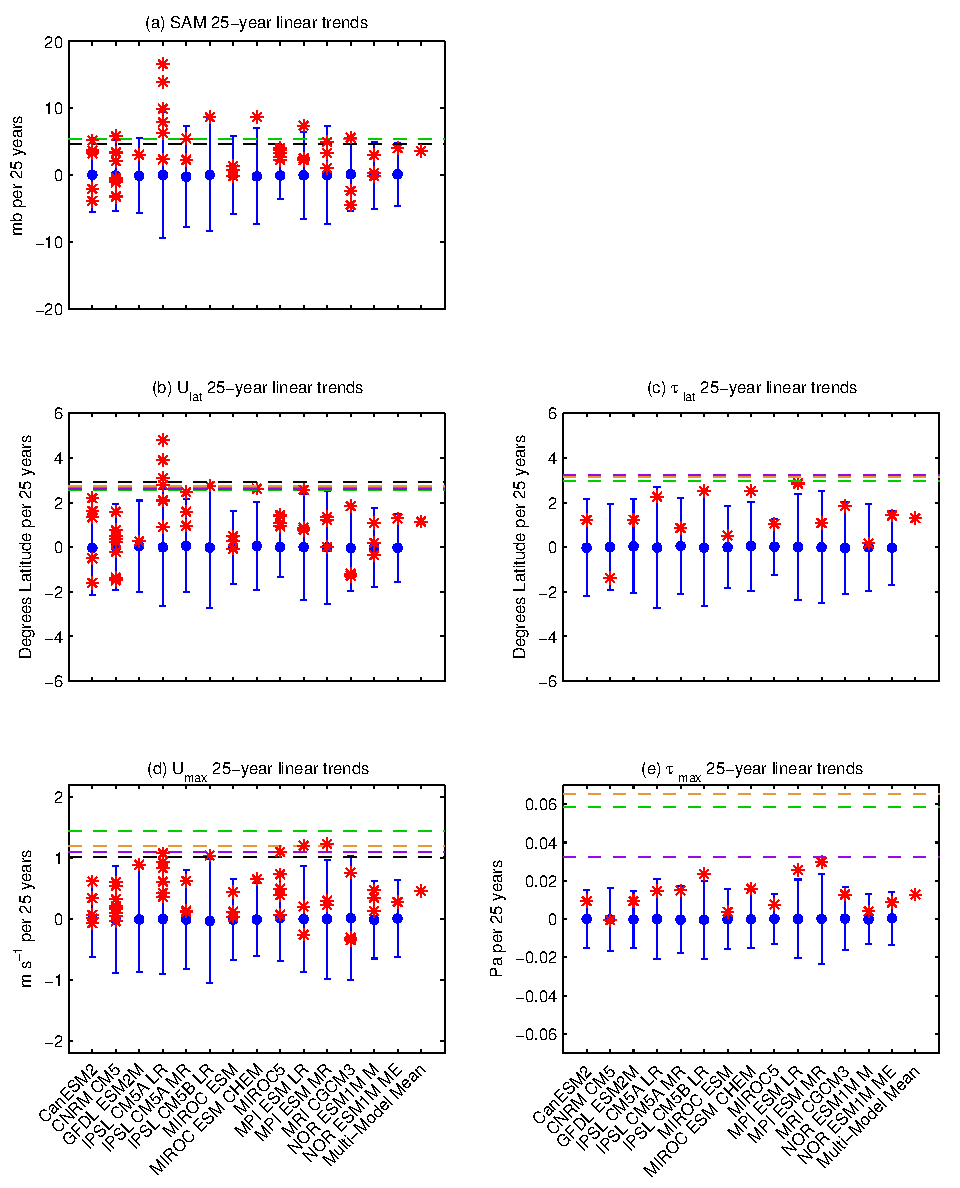
\includegraphics[width=1\linewidth]{figures/chapter-SHcirc/2014jgrl-p02.pdf}
\caption{Natural variability, historical trends and observations for (a) SAM,
(b) 850mb jet latitude, (c) wind-stress jet latitude, (d) 850mb jet magnitude,
and (e) wind-stress jet magnitude. Blue circles show the mean of the piControl
25-year linear trends indicating model drift. Whisker length is 2 standard
deviations. Red points show the historical run trends for each ensemble member.
Horizontal dashed lines indicate the absolute value of the observed trends: NCEP
R1 (green), NCEP R2 (orange), ERA-Int (purple), and JRA-55 (black).}
\label{fig:ch2_fig2}
\end{figure}

The observed SAM trend observations lie just within the whiskers for most of the
models, indicating the observed trends lie within the model natural variability.
To quantify this further, the probability of each model randomly obtaining a
trend with the magnitude of the average reanalysis SAM trend or larger is shown
in table 2 (column 1). 10 of the 14 models have a probability of 5\% or greater,
and thus there is a significant (at the 5\% level) probability of  obtaining the
observed 25-year trend in the piControl simulations by chance alone. In other
words, the observed trend over the period 1980-2004 in the SAM lies just within
the edge of natural variability as described by these models. This result also
holds for the period 1980-2014 (not shown).

The observed $\tau_{lat}$ and $U_{lat}$ trends are just outside the model's
natural decadal variability (Figure 2b and c).  If we calculate the probability
of each model obtaining the observed average reanalysis $U_{lat}$ trend (table
2, column 2), then we see that no models have a probability of 5\% or greater;
however, 6 of the 14 have greater than a 1\% probability. Thus, there is not a
significant (at the 5\% level) probability of obtaining the observed trend using
natural variability alone.

In contrast, the observed trends in $\tau_{max}$ and $U_{max}$ are both outside
the natural variability as described by the models (Figure 2d and e). The
probability of obtaining the average reanalysis $U_{max}$ trend in all but one
of the piControl models is less than 1\% (table 2, column 3) and therefore there
is not a significant (at the 1\% level) probability of the natural variability
reproducing the observed trend. The probabilities of the piControl $\tau_{max}$
and $\tau_{lat}$ obtaining the observed trends are not shown in table 2, but are
consistent with the $U_{max}$ and $U_{lat}$ probabilities.

The above shows that the observed trends in the SAM largely lie at the edge of
natural multi-decadal variability of the piControl model runs. However, this
does not necessarily mean that the observed trends are not forced by
anthropogenic activities, merely that the observations can contain a large
component of natural variability in the SAM. The observed trend in the jet
location and magnitude, however, is outside the variability of most models
piControl runs. This does suggest an external force driving the jet to
strengthen and shift over this 25-year period.

\subsection{Model historical trends}

We now examine the model historical runs to understand how the modeled trends
compare to the modeled natural variability and to compare the modeled trends
with the observed trends. The red asterisks in Figure 2 represent the 25-year
trend for each historical run (the number of historical runs varies among the
models).

There is considerable variability amongst the models in the magnitude of the
trends, but for all five metrics the vast majority of the simulated historical
trends are of the same sign (increase in SAM, poleward shift and strengthening
of the jet). This consistency in sign indicates that external (anthropogenic)
forcing is causing at least part of the trend.  However,  the magnitude of the
historical trends are almost all within the natural multi-decadal variability of
the corresponding model (i.e. within the whiskers). Thus while the response in
the models between 1980 and 2004 is due (at least in part) to forcing, the
response does not overwhelm the natural variability.

For the SAM, the magnitude of the individual historical ensemble member trends
are largely within the estimated natural variability and highly variable, with
some ensemble members having trends of the opposite sign to the observations
(dashed horizontal lines). Because the observed trends are generally within the
natural decadal variability of the models a close agreement between individual
historical ensemble members and observed trends would not be expected due to the
high component of natural variability. Most of the ensemble members have
positive trends and the magnitude of the multi-model ensemble mean historical
trend is similar to the observations. This further suggests an anthropogenic
forcing pushing the SAM towards positive phase.

The same comparison for jet location and magnitude yields different results.
The observed trends in the jet metrics are outside the natural variability of
the models, and generally larger than the modeled historical trends (especially
for the magnitude of the wind stress). A possible cause for this is that the
observed trends are due to anthropogenic forcing that is not well represented
(or under represented) in the models.  However, another possibility is that
there are issues with the reanalyses and the reanalyses are overestimating the
real trend.  This may especially be the case for the NCEP reanalyses, where the
wind stress trends  are significantly outside the model natural variability but
the 850 hPa winds are just outside the model natural variability.

If we consider the observed trends to be a combination of natural variability
and external forcing, and if we use the ensemble-mean historical trend as a
representation of the forced response, we can better capture the observed trend.
The last 3 columns in table 2 show the probability of obtaining the mean
reanalysis trend from a combination of each model's natural variability and the
multi-model ensemble mean historical trend (results for $\tau_{lat}$ and
$\tau_{max}$ are not shown, but are consistent with $U_{lat}$ and $U_{max}$).
The probabilities for each metric are substantially greater, indicating that
there is a significant probability, in most models, that the observed trends are
due to this combination of natural variability and anthropogenic forcing. This
does not exclude the possibility that the models are systematically biased low,
or that the reanalyses are biased high, but it suggests that the mismatch is
smaller than might be suggested from previous work \citep{Swart2012a}.

\begin{figure}
\noindent
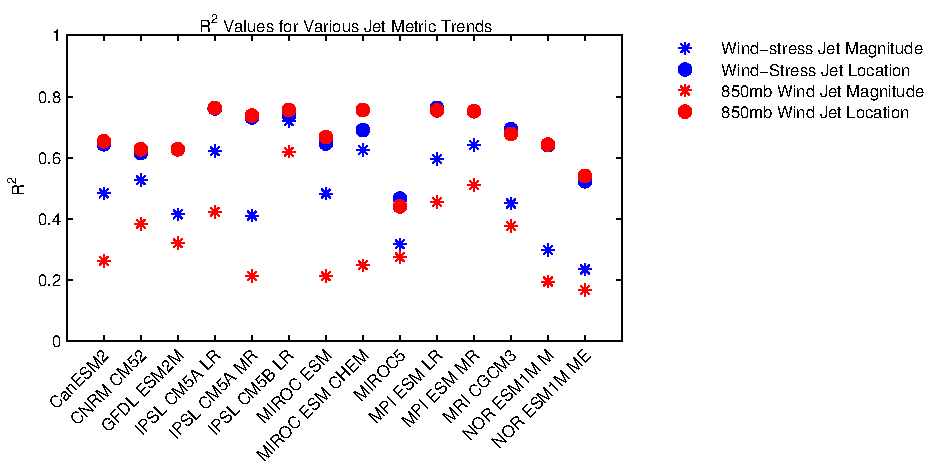
\includegraphics[width=0.9\linewidth]{figures/chapter-SHcirc/2014jgrl-p03.pdf}
\label{fig:ch2_fig3}
\caption{Correlation coefficient squared for correlation of the the 25-year
linear trends in wind-stress jet location, wind-stress jet magnitude, 850mb jet
location, and 850mb jet magnitude with the 25-year trends in SAM for each model.}
\end{figure}


\section{Conclusions}

Changes in the SAM are often linked with concurrent changes in the SH westerly
jet magnitude and location [\textit{Hall \& Visbeck}, 2002]. Additionally,
observational studies have shown recent trends in these diagnostics and
attribute them to a combination of ozone depletion and greenhouse gas induced
warming \citep{Arblaster2006}. By comparing CMIP5 models piControl and
historical runs with reanalysis observations, we have shown that there are
significant differences in the observed and modeled trends of the SAM from those
in the jet. Hence, the SAM and jet metrics cannot be used interchangeably.

Examining the natural variability of the SAM using CMIP5 preindustrial control
runs has led to the conclusion that the observed trend is not decisively outside
the natural variability as simulated by the CMIP5 models. While the modeled
natural variability in SAM in quite large, the positive bias of the model
historical trends suggest influence of an external forcing. The failure of
individual historical models to simulate the magnitude of the observed
historical trend could be due to the natural variability and not deficiencies in
the simulations.

In contrast, the observed trends in jet location and magnitude are outside the
natural variability of the models. The historical model runs also seem to
underestimate the magnitude of these trends, especially in jet magnitude.
Combining the natural variability and historical trend brings the models closer
to capturing the observed trends in jet location and magnitude, but this does
not eliminate the possibility that the model trends are biased low or the
reanalyses are biased high.

Changes in the SAM and SH westerly jet have been linked with significant changes
in ocean circulation, ocean heat and carbon uptake \citep{Mignone2006b}, and
Antarctic sea-ice extent \citep{Fan2014b}. We suggest that changes
in SAM and jet latitude may behave differently than changes in jet magnitude and
thus may have independent effects on the Southern Ocean and Antarctic climate.
Understanding how these atmospheric variables interact with each other will be
critical for predicting the future evolution of ocean circulation and the earth
system.


%\bibliography{/RESEARCH/library}
%%% Local Variables:
%%% mode: latex
%%% TeX-master: "thesis"
%%% End:
